%!TEX root = ../konzept.tex

\section{Kommunikationsabläufe und Interaktionen}

Zur Festlegung der Systemarchitektur werden zunächst die Anforderungen anhand eines möglichen Kommunikationsablaufs eines erfolgreichen Interaktionsszenario betrachtet (Abb. \ref{kommunkationsablauf}).\\

Ein potentieller Mieter nutzt die Smartphone-Anwendung zunächst um seinen eigenen Standort zu ermitteln. Daraufhin sendet er seine Anfrage an unser Hauptsystem, welches das erste \textit{Matching} durchführt.

In einer Datenbank befinden sich Zuordnungen zwischen Vermieter und dem Ort eines Mietobjektes. Auf Basis diese Datenmenge wird ein Abgleich zwischen angefragtem Ort und vorhandenen Orten durchhgeführt. Bei allen möglichen Treffern wird der zugehörige Nutzer herausgefiltert.

Zu den relevanten Daten eines Nutzers gehört unter anderem eine Identifikationsnummer, unter welcher das Smartphone des Vermieters ansprechbar ist. Dadurch werden die nun gefilterten Vermieter angesprochen und bekommen ein Ereignis zugesendet.

Das Ereignis beinhaltet die relevanten Daten der Anfrage durch den Mieter. Sobald das Ereignis das Ziel erreicht hat, wird auf dem Endgerät des Vermieters das zweite \textit{Matching} durchgeführt, denn wie in der Martkanalyse bereits identifiziert wurde, werden direkte Personen- und Objektdaten auf den Endgeräten der Nutzer gespeichert.

Der zweite Abgleich vergleicht also das gesendete Profil mit dem auf dem Gerät gespeicherten Profil. Ein Algorithmus berechnet dabei die

\begin{figure}[H]
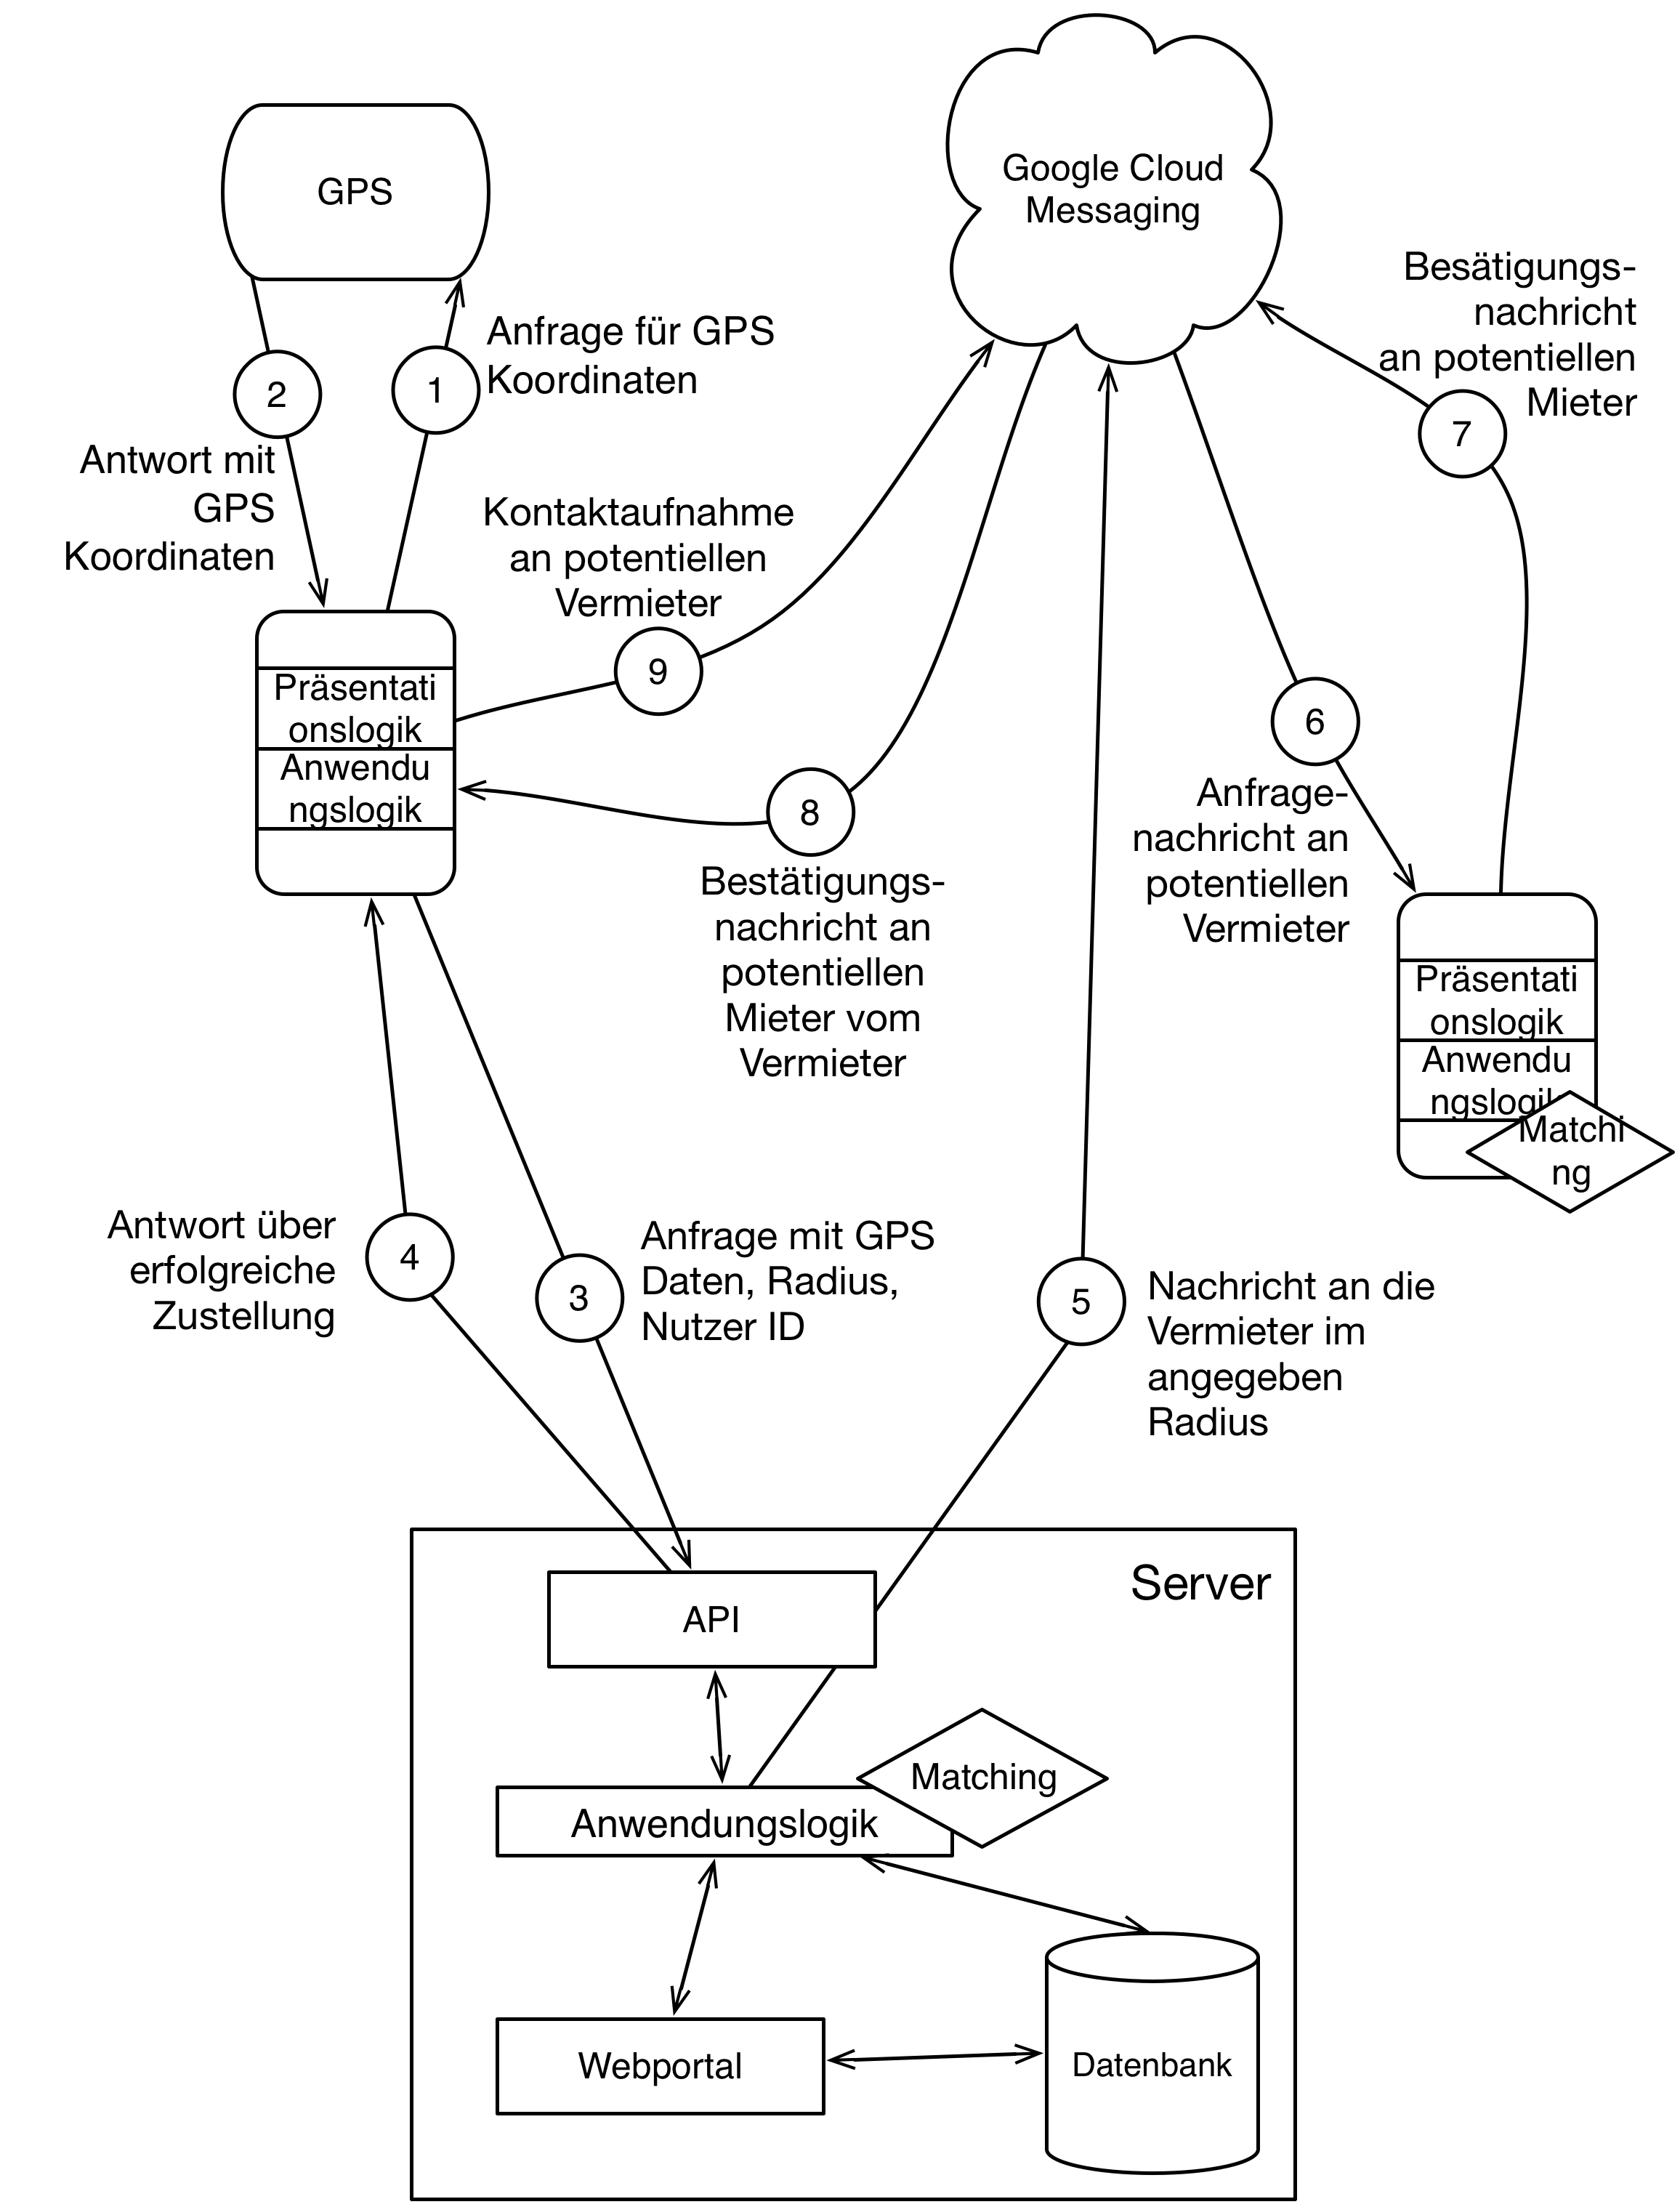
\includegraphics[width=.9\textwidth]{./images/kommunkationsablauf.png}
\caption{Kommunkationsablauf eines möglichen Erfolgsszenrario}
\label{kommunkationsablauf}
\end{figure}


Für die Analyse zunächst ein Überblick über die möglichen Architektur-Paradigmen, mit einer ersten Abwägung.\\

\textbf{Publish-Subscribe}\\


Entfernte Prozedur- und Methodenaufrufe => Polling

WS* Architektur


Lose Kopplung
